% chktex-file 2% chktex-file 29
% chktex-file 13
\documentclass[12pt]{report}
\usepackage{setspace}
\usepackage[a4paper, total={7in, 10in}]{geometry}
\usepackage[fleqn]{amsmath}
\usepackage{empheq}
\usepackage{amssymb}
\usepackage{amsthm}
\usepackage{gensymb}
\usepackage[fleqn]{cases}
\usepackage{multicol}
\usepackage{color}
\usepackage{stix}
\usepackage{chngcntr}
\usepackage{tikz}
\usepackage{enumitem}
\usepackage{pgfplots}
\usepackage{etoolbox}
\usepackage{tkz-euclide}
\usepackage{graphicx}
\usepackage{enumitem}
\usepackage{multirow}
\usepackage{mathtools}
\usepackage{mdframed}
\usepackage{adjustbox}
\usepackage{xpatch}
\usepackage{nicematrix}
\usepackage{ifthen}

\def\nswe#1#2#3{#1\,$#2^\circ\,#3'$}
\graphicspath{ {./assets/} }
\usetikzlibrary{calc,trees,positioning,arrows,fit,shapes,calc, decorations.markings}
\newcommand{\midarrow}{\tikz \draw[-triangle 90] (0,0) -- +(.1,0);}

\newcommand\typel[2]{
    \mathbin{\mathop{#1\kern0pt}%
        \limits_{\raisebox{3.6ex}{\hbox to0pt{\hss\strut$\uparrow$\hss}}\hbox to0pt{\hss#2\hss}}}
}

\newcommand\typem[2]{
    \mathbin{\mathop{#1\kern0pt}%
        \limits^{\raisebox{3.6ex}{\hbox to0pt{\hss#2\hss}}\hbox to0pt{\hss\strut$\downarrow$\hss}}}
}

\counterwithout{equation}{chapter}

\newcommand{\pgfplotsdrawaxis}{\pgfplots@draw@axis}
\newcommand\perm[2][^n]{\prescript{#1\mkern-2.5mu}{}P_{#2}}
\newcommand\permtwo[2][^n]{{}_{#1}P_{#2}}
\newcommand\comb[2][^n]{{}_{#1}C_{#2}}
\newcommand\combtwo[2][^n]{\prescript{#1\mkern-2.5mu}{}C_{#2}}
\makeatother
\pgfplotsset{only axis on top/.style={axis on top=false, after end axis/.code={
                    \pgfplotsset{axis line style=opaque, ticklabel style=opaque, tick style={thick,opaque},
                        grid=none}\pgfplotsdrawaxis}}}

\newtheorem{theorem}{Theorem}

\makeatletter
\xpatchcmd{\endmdframed}
{\aftergroup\endmdf@trivlist\color@endgroup}
{\endmdf@trivlist\color@endgroup\@doendpe}
{}{}
\makeatother

\mdfdefinestyle{MyFrame}{%
    linecolor=black,
    linewidth=1pt,
    roundcorner=20pt, innertopmargin=20pt,innerbottommargin=20pt, innerrightmargin=12pt,
    innerleftmargin=12pt, skipbelow=20pt, skipabove=20pt
    %backgroundcolor=gray!50!white}
}

\newcommand{\newitem}[1]{%
    \refstepcounter{subenum}%
    \parbox{\dimexpr.5\linewidth-.5\columnsep}{
        \makebox[\labelwidth][r]{(\thesubenum)\hspace*{\labelsep}} #1}\hfill }%%%

\setcounter{chapter}{21}

\setlength{\arrayrulewidth}{1pt}
\setlength{\tabcolsep}{12pt}

\begin{document}

\newcommand{\sol}[1]{

    \noindent \textbf{Sol.}
}
\newcommand{\prooff}[1]{

    \noindent \textbf{Proof.}
}

\newcommand{\sxrightarrow}[2][]{%
    \mathrel{\text{$\xrightarrow[#1]{#2}$}}%
}

\newenvironment{cequation}{
    \makeatletter
    \setbool{@fleqn}{false}
    \makeatother
    \begin{equation*}
        }{\end{equation*}}

\begin{titlepage}
    \raggedleft{}
    \rule{1pt}{\textheight}
    \hspace{0.02\textwidth}
    \parbox[b]{0.75\textwidth}{

    {\fontsize{40}{60}\selectfont\bfseries Mathematics}\\[2\baselineskip]
    {\huge\textit{Senior 3 Part I}}\\[4\baselineskip]
    {\Large\textsc{Melvin Chia}}

    \vspace{0.5\textheight}

    {\noindent Started on 10 April 2023}\\[\baselineskip]
    {\noindent Finished on XX XX 2023}\\[\baselineskip]
    {\noindent Actual time spent: XX days}\\[\baselineskip]}

\end{titlepage}

\chapter*{Introduction}
\addcontentsline{toc}{chapter}{Introduction} \markboth{INTRODUCTION}{}

\doublespacing{}
\section*{Why this book?}

\section*{Disclaimer}
\section*{Acknowledgements}

\singlespacing{}

\doublespacing{}
\tableofcontents
\singlespacing{}
\newpage

\onehalfspacing

\section*{Revision Exercise 22}

\begin{enumerate}
    \item Determine whether the following mappings from set $A = \{1, 2, 3, 4\}$ to set
          $B = \{a, b, c, d\}$ are functions or not.
          \begin{enumerate}
              \item $1 \to a$, $2 \to c$, $4 \to b$
                    \sol{}

                    Since $3 \in A$ does not have an image in $B$, this is not a function.

              \item $1 \to a$, $2 \to d$, $3 \to b$, $4 \to a$
                    \sol{}

                    Since each element in $A$ has an image in $B$, this is a function.

              \item $1 \to c$, $2 \to c$, $3 \to b$, $4 \to b$
                    \sol{}

                    Since each element in $A$ has an image in $B$, this is a function.

              \item $1 \to a$, $2 \to c$, $2 \to b$, $4 \to d$
                    \sol{}

                    Since $2 \in A$ has two images $b$ and $c$ in $B$, $3 \in A$ has two images in
                    $B$, this is not a function.

              \item $1 \to c$, $2 \to b$, $3 \to d$, $4 \to c$, $4 \to a$
                    \sol{}

                    Since $4 \in A$ has two images $c$ and $a$ in $B$, this is not a function.
          \end{enumerate}

    \item Given the function $f: \mathbb{R} \to \mathbb{R}$ be defined by $f(x) = \left\{\begin{array}{rl}
                  3x - 2,   & x < -3        \\
                  2x^2 + 4, & -3 \leq x < 2 \\
                  -2x + 9,  & x \geq 2
              \end{array}\right.$, find
          \begin{enumerate}
              \begin{multicols}{2}
                  \item $f(-4)$
                  \sol{}
                  \begin{flalign*}
                      f(-4) & = 3(-4) - 2 \\
                            & = -14
                  \end{flalign*}

                  \item $f(0)$
                  \sol{}
                  \begin{flalign*}
                      f(0) & = 2(0)^2 + 4 \\
                           & = 4
                  \end{flalign*}
              \end{multicols}
              \begin{multicols}{2}
                  \item $f(2)$
                  \sol{}
                  \begin{flalign*}
                      f(2) & = -2(2) + 9 \\
                           & = 5
                  \end{flalign*}

                  \item $f(3)$
                  \sol{}
                  \begin{flalign*}
                      f(3) & = -2(3) + 9 \\
                           & = 3
                  \end{flalign*}
              \end{multicols}
          \end{enumerate}

          \newpage
    \item Find the domain and range of the following functions:
          \begin{enumerate}
              \item $f: 1 \to 3$, $2 \to 5$, $4 \to 8$
                    \sol{}

                    $D_f = \{1, 2, 4\}$, $R_f = \{3, 5, 8\}$

              \item $g: 2 \to 4$, $4 \to 5$, $5 \to 7$, $6 \to 9$
                    \sol{}

                    $D_g = \{2, 4, 5, 6\}$, $R_g = \{4, 5, 7, 9\}$

              \item $h: 1 \to 3$, $2 \to 5$, $3 \to 6$, $4 \to 8$
                    \sol{}

                    $D_h = \{1, 2, 3, 4\}$, $R_h = \{3, 5, 6, 8\}$
          \end{enumerate}

    \item The table below shows a function $f$:
          \begin{center}
              \begin{NiceTabular}{|c|c|c|c|c|c|}[hvlines,cell-space-limits=5pt, code-before = \rectanglecolor{lightgray!50}{1-1}{2-1}]
                  x    & -3  & -2 & -1 & 0 & 1 \\
                  f(x) & -22 & -3 & 4  & 5 & 6 \\
              \end{NiceTabular}
          \end{center}
          \begin{enumerate}
              \item Find the domain and range of the function; \sol{}

                    $D_f = \{-3, -2, -1, 0, 1\}$, $R_f = \{-22, -3, 4, 5, 6\}$

              \item Express the function using graph. \sol{}
                    \begin{center}
                        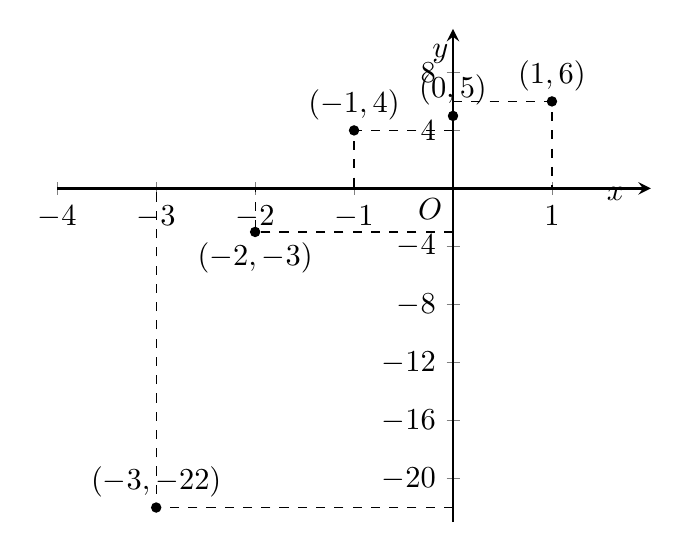
\begin{tikzpicture}[scale=1.1]
                            \begin{axis}[
                                    axis lines = middle,
                                    xlabel = $x$,
                                    ylabel = {$y$},
                                    ymin = -23,
                                    ymax = 11,
                                    xmin = -4,
                                    xmax = 2,
                                    xtick = {-4, -3, ..., 1},
                                    ytick = {-24, -20, ..., 12},
                                    xlabel style={below right, xshift=-1.8em, yshift=0.4em},
                                    ylabel style={above left, xshift=0.2em, yshift=-1.5em},
                                    axis line style={thick}
                                ]

                                \node at (axis cs:0,0) [anchor=north east] {$O$};

                                \filldraw[black] (axis cs:-3,-22) circle (1.5pt) node [above] {$(-3,-22)$};
                                \filldraw[black] (axis cs:-2,-3) circle (1.5pt) node [below] {$(-2,-3)$};
                                \filldraw[black] (axis cs:-1,4) circle (1.5pt) node [above] {$(-1,4)$};
                                \filldraw[black] (axis cs:0,5) circle (1.5pt) node [above] {$(0,5)$};
                                \filldraw[black] (axis cs:1,6) circle (1.5pt) node [above] {$(1,6)$};

                                \draw[dashed] (axis cs: 0, -22) -- (axis cs: -3, -22) -- (axis cs: -3, 0);
                                \draw[dashed] (axis cs: 0, -3) -- (axis cs: -2, -3) -- (axis cs: -2, 0);
                                \draw[dashed] (axis cs: 0, 4) -- (axis cs: -1, 4) -- (axis cs: -1, 0);
                                \draw[dashed] (axis cs: 0, 5) -- (axis cs: 0, 5) -- (axis cs: 0, 0);
                                \draw[dashed] (axis cs: 0, 6) -- (axis cs: 1, 6) -- (axis cs: 1, 0);
                            \end{axis}
                        \end{tikzpicture}
                    \end{center}

              \item Determine if the inverse function of $f$ exists. \sol{}

                    Since each element in the codomain of $f$ is mapped to exactly one element in
                    the domain of $f$, the function $f$ is a one-to-one function. Since each
                    element in the codomain of $f$ has preimage in the domain of $f$, the function
                    $f$ is an onto function.

                    Hence, the function $f$ is a one to one onto function. According to the
                    definition of inverse function, the inverse function of $f$ exists.
          \end{enumerate}

    \item As shown in the diagram below, let a function $f: x \to ax + b$. Find the value
          of $f(4)$ and $f^{-1}(5)$.
          \begin{center}
              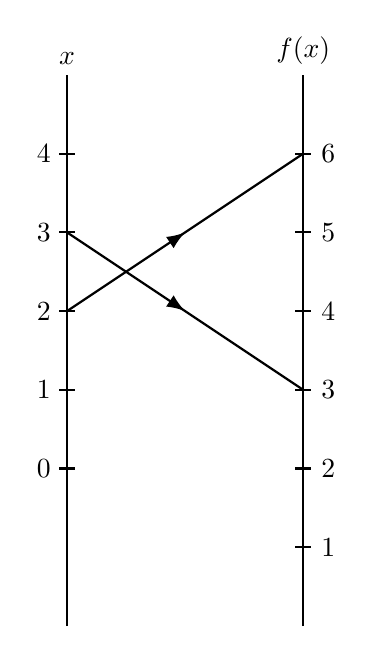
\begin{tikzpicture}
                  \draw[thick] (0,0) -- (0,7) node[above]{$x$};
                  \draw[thick] (3,0) -- (3,7) node[above]{$f(x)$};
                  \draw[thick] (-0.1,2) -- (0.1,2) node[left=5pt]{$0$};
                  \draw[thick] (-0.1,3) -- (0.1,3) node[left=5pt]{$1$};
                  \draw[thick] (-0.1,4) -- (0.1,4) node[left=5pt]{$2$};
                  \draw[thick] (-0.1,5) -- (0.1,5) node[left=5pt]{$3$};
                  \draw[thick] (-0.1,6) -- (0.1,6) node[left=5pt]{$4$};
                  \draw[thick] (2.9,1) -- (3.1,1) node[right]{$1$};
                  \draw[thick] (2.9,2) -- (3.1,2) node[right]{$2$};
                  \draw[thick] (2.9,3) -- (3.1,3) node[right]{$3$};
                  \draw[thick] (2.9,4) -- (3.1,4) node[right]{$4$};
                  \draw[thick] (2.9,5) -- (3.1,5) node[right]{$5$};
                  \draw[thick] (2.9,6) -- (3.1,6) node[right]{$6$};
                  \begin{scope}[thick,decoration={
                                  markings,
                                  mark=at position 0.5 with {\arrow{Latex}}}
                      ]
                      \draw[postaction={decorate}] (0, 4) -- (3, 6);
                      \draw[postaction={decorate}] (0, 5) -- (3, 3);
                  \end{scope}
              \end{tikzpicture}
          \end{center}
          \sol{}
          \vspace{-1cm}
          \begin{multicols}{2}
              \begin{flalign*}
                  f(3)             & = 3a + b = 3     \\
                  f(2)             & = 2a + b = 6     \\
                  f(3) - f(2)      & = a = -3         \\
                  3(-3) + b        & = 3              \\
                  b                & = 12             \\
                  \\
                  \therefore\ f(x) & = -3x + 12       \\
                  \\
                  f(4)             & = -3(4) + 12 = 0
              \end{flalign*}

              \begin{flalign*}
                  \text{Let } y         & = f^{-1}(x)           \\
                  f(y)                  & = x                   \\
                  -3y + 12              & = x                   \\
                  y                     & = -\dfrac{x - 12}{3}  \\
                  \\
                  \therefore\ f^{-1}(x) & = -\dfrac{x - 12}{3}  \\
                  f^{-1}(5)             & = -\dfrac-{5 - 12}{3} \\
                                        & = \dfrac{7}{3}
              \end{flalign*}
          \end{multicols}

    \item Given the function $f:x \to x^2 - x + 1$, $-1 \leq x \leq 3$, find its range.
          \sol{} \vspace{-3em}
          \begin{multicols}{2}
              \begin{flalign*}
                  f(x)          & = x^2 - x + 1                                    \\
                                & = \left(x - \dfrac{1}{2}\right)^2 + \dfrac{3}{4} \\
                  \text{Vertex} & : \left(\dfrac{1}{2}, \dfrac{3}{4}\right)        \\
                  \because\ a   & > 0, y_{\min} = \dfrac{3}{4}                     \\
              \end{flalign*}

              \begin{flalign*}
                  f(-1)           & = (-1)^2 - (-1) + 1 = 3                                           \\
                  f(3)            & = 3^2 - 3 + 1 = 7                                                 \\
                  \\
                  \therefore\ R_f & = \left\{y | y \in \mathbb{R}, \dfrac{3}{4} \leq y \leq 7\right\}
              \end{flalign*}
          \end{multicols}

          \newpage
    \item Let function $f:x \to 2x^2 - 4x + 3$.
          \begin{enumerate}
              \item If $D_f = \mathbb{R}$, find the range of $f$; \sol{}
                    \begin{flalign*}
                        f(x)            & = 2x^2 - 4x + 3                                 \\
                                        & = 2(x^2 - 2) + 3                                \\
                                        & = 2(x-1)^2 +1                                   \\
                        \text{Vertex}   & : (1, 1)                                        \\
                        \because\ a     & > 0, y_{\min} = 1
                        \\
                        \therefore\ R_f & = \left\{y | y \in \mathbb{R}, y \geq 1\right\}
                    \end{flalign*}

              \item If $D_f = \left\{x | x \geq 3\right\}$, find the range of $f$. \sol{}
                    \begin{flalign*}
                        f(3)            & = 2(3)^2 - 4(3) + 3 = 9                         \\
                        \therefore\ R_f & = \left\{y | y \in \mathbb{R}, y \geq 9\right\}
                    \end{flalign*}
          \end{enumerate}

    \item Find the domain and range of the following functions:
          \begin{enumerate}
              \begin{multicols}{2}
                  \item $f(x) = \dfrac{1}{x}$
                  \sol{}

                  $\because\ f(x)$ is defined when $x \neq 0$,

                  $\therefore\ D_f = \mathbb{R} \setminus \{0\}$.

                  $\because\ f(x) = \dfrac{1}{x} \neq 0$,

                  $\therefore\ R_f = \mathbb{R} \setminus \{0\}$.

                  \item $f(x) = \sqrt{2x - 5}$
                  \sol{}

                  $\because\ f(x)$ is defined when $2x - 5 \geq 0$,

                  $\therefore\ D_f = \left\{x | x \geq \dfrac{5}{2}\right\}$.

                  $\because\ f(x) = \sqrt{2x - 5} \geq 0$,

                  $\therefore\ R_f = \left\{y | y \geq 0\right\}$.
              \end{multicols}

              \begin{multicols}{2}
                  \item $f(x) = x^2 + 4x + 7$
                  \sol{}

                  $\because\ f(x)$ is defined for all $x \in \mathbb{R}$,\\
                  $\therefore\ D_f = \mathbb{R}$.
                  \begin{flalign*}
                      f(x)            & = x^2 + 4x + 7                                  & \\
                                      & = (x + 2)^2 + 3                                   \\
                      \text{Vertex}   & : (-2, 3)                                         \\
                      \because\ a     & > 0, y_{\min} = 3                                 \\
                      \\
                      \therefore\ R_f & = \left\{y | y \in \mathbb{R}, y \geq 3\right\}
                  \end{flalign*}

                  \item $f(x) = \dfrac{1}{x^2 + 4}$
                  \sol{}
                  $\because\ x^2 + 4 \geq 4$ for all $x \in \mathbb{R}$,\\

                  $\therefore\ D_f = \mathbb{R}$.

                  $\because\ f(x) = x^2 + 4 \geq 4$ for all $x \in \mathbb{R}$,\\

                  $\therefore\ f(x) \geq \dfrac{1}{4}$ for all $x \in \mathbb{R}$,\\

                  $\therefore\ R_f = \left\{y | y \in \mathbb{R}, y \geq \dfrac{1}{4}\right\}$.
              \end{multicols}
          \end{enumerate}

    \item Find the domain of the following functions:
          \begin{enumerate}
              \begin{multicols}{2}
                  \item $f(x) = \dfrac{2x}{x-3}$
                  \sol{}

                  $\because\ f(x)$ is defined when $x - 3 \neq 0$,

                  $\therefore\ D_f = \mathbb{R} \setminus \{3\}$.

                  \item $f(x) = \sqrt{4 - x^2}$
                  \sol{}

                  $\because\ f(x)$ is defined when $4 - x^2 \geq 0$,

                  $\therefore\ D_f = \left\{x | x \in \mathbb{R}, -2 \leq x \leq 2\right\}$.
              \end{multicols}
              \begin{multicols}{2}
                  \item $f(x) = \dfrac{x-2}{2x^2 - 5x + 2}$
                  \sol{}

                  $\because\ f(x)$ is defined when $2x^2 - 5x + 2 \neq 0$,

                  $\therefore\ D_f = \left\{x | x \in \mathbb{R}, x \neq \dfrac{1}{2}, x \neq 2\right\}$.

                  \item $f(x) = \dfrac{x-3}{\sqrt{x^2 - 9}}$
                  \sol{}

                  $\because\ f(x)$ is defined when $x^2 - 9 > 0$,

                  $\therefore\ D_f = \left\{x | x \in \mathbb{R}, x < -3 \text{ or } x > 3\right\}$.
              \end{multicols}
          \end{enumerate}

    \item Sketch the graph for the following functions:
          \begin{enumerate}
              \item $f(x) = 2x^2 - 5x + 9$
                    \sol{}
                    \begin{center}
                        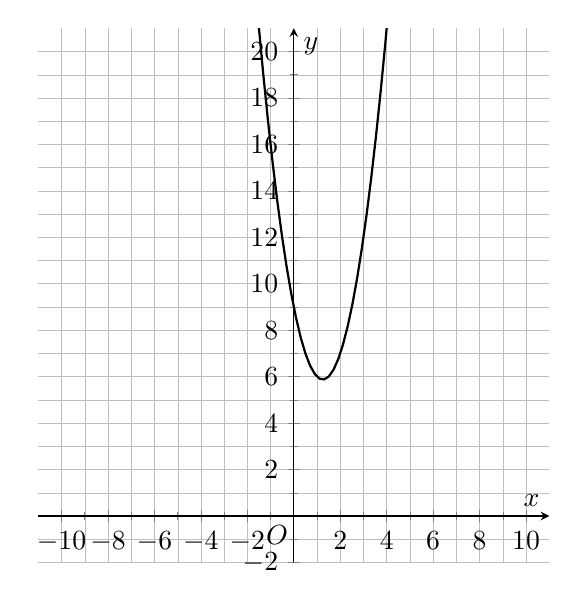
\begin{tikzpicture}
                            \begin{axis}[
                                    unit vector ratio*=1 1 1,
                                    axis lines = middle,
                                    xlabel = $x$,
                                    ylabel = $y$,
                                    ymin = -2,
                                    ymax = 21,
                                    xmin = -11,
                                    xmax = 11,
                                    xtick = {-10, -8,...,10},
                                    ytick = {-2,0,...,20},
                                    minor tick num = 1,
                                    grid = both,
                                    grid style = {line width=.1pt, draw=gray!50},
                                    major grid style = {line width=.2pt,draw=gray!50},
                                    width = 0.8\textwidth,
                                ]
                                \node at (axis cs: 0,0) [anchor=north east, xshift=0.05cm] {$O$};
                                \addplot [
                                    thick,
                                    domain=-10:10,
                                    samples=100,
                                ]
                                {2*x^2 - 5*x + 9};
                            \end{axis}
                        \end{tikzpicture}
                    \end{center}
                    \newpage

              \item $f(x) = -3x^2 + 6x + 11$
                    \sol{}
                    \begin{center}
                        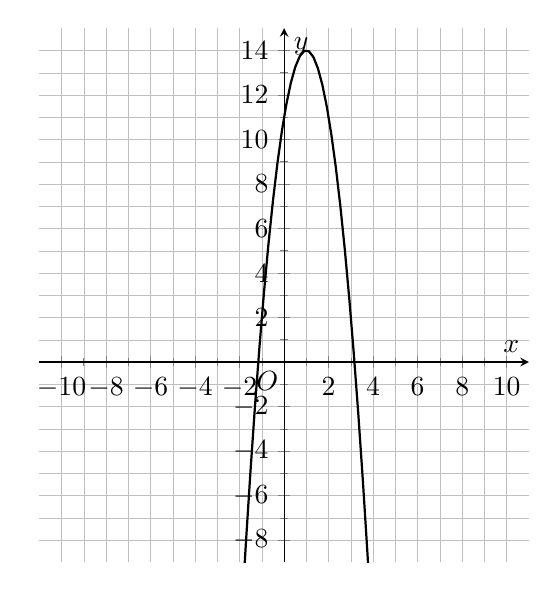
\begin{tikzpicture}
                            \begin{axis}[
                                    unit vector ratio*=1 1 1,
                                    axis lines = middle,
                                    xlabel = $x$,
                                    ylabel = $y$,
                                    ymin = -9,
                                    ymax = 15,
                                    xmin = -11,
                                    xmax = 11,
                                    xtick = {-10, -8,...,10},
                                    ytick = {-8,-6,...,14},
                                    minor tick num = 1,
                                    grid = both,
                                    grid style = {line width=.1pt, draw=gray!50},
                                    major grid style = {line width=.2pt,draw=gray!50},
                                    width = 0.8\textwidth,
                                ]
                                \node at (axis cs: 0,0) [anchor=north east, xshift=0.05cm] {$O$};
                                \addplot [
                                    thick,
                                    domain=-10:10,
                                    samples=100,
                                ]
                                {-3*x^2 + 6*x + 11};
                            \end{axis}
                        \end{tikzpicture}
                    \end{center}

              \item $f(x) = 3x^2 + 12x + 10$
                    \sol{}
                    \begin{center}
                        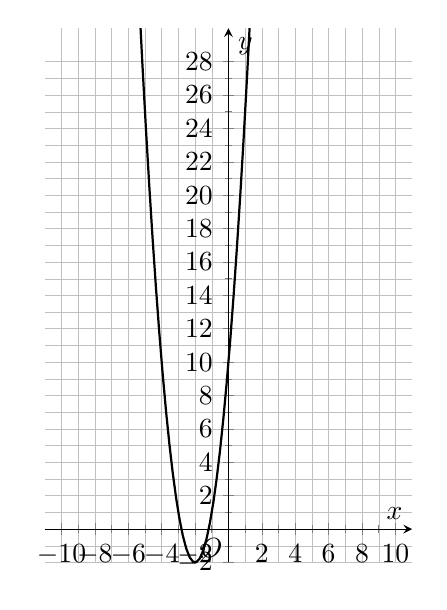
\begin{tikzpicture}
                            \begin{axis}[
                                    unit vector ratio*=1 1 1,
                                    axis lines = middle,
                                    xlabel = $x$,
                                    ylabel = $y$,
                                    ymin = -2,
                                    ymax = 30,
                                    xmin = -11,
                                    xmax = 11,
                                    xtick = {-10, -8,...,10},
                                    ytick = {-2,0,...,28},
                                    minor tick num = 1,
                                    grid = both,
                                    grid style = {line width=.1pt, draw=gray!50},
                                    major grid style = {line width=.2pt,draw=gray!50},
                                    width = 0.8\textwidth,
                                ]
                                \node at (axis cs: 0,0) [anchor=north east, xshift=0.05cm] {$O$};
                                \addplot [
                                    thick,
                                    domain=-10:10,
                                    samples=100,
                                ]
                                {3*x^2 + 12*x + 10};
                            \end{axis}
                        \end{tikzpicture}
                    \end{center}

              \item $f(x) = -5x^2 + 6x + 11$
                    \sol{}
                    \begin{center}
                        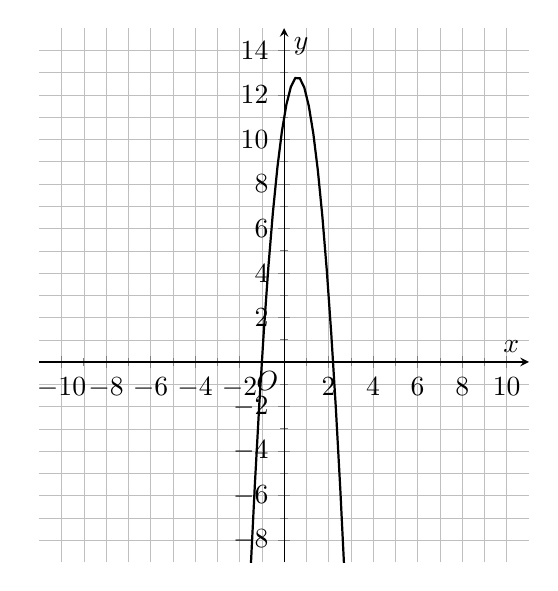
\begin{tikzpicture}
                            \begin{axis}[
                                    unit vector ratio*=1 1 1,
                                    axis lines = middle,
                                    xlabel = $x$,
                                    ylabel = $y$,
                                    ymin = -9,
                                    ymax = 15,
                                    xmin = -11,
                                    xmax = 11,
                                    xtick = {-10, -8,...,10},
                                    ytick = {-8,-6,...,14},
                                    minor tick num = 1,
                                    grid = both,
                                    grid style = {line width=.1pt, draw=gray!50},
                                    major grid style = {line width=.2pt,draw=gray!50},
                                    width = 0.8\textwidth,
                                ]
                                \node at (axis cs: 0,0) [anchor=north east, xshift=0.05cm] {$O$};
                                \addplot [
                                    thick,
                                    domain=-10:10,
                                    samples=100,
                                ]
                                {-5*x^2 + 6*x + 11};
                            \end{axis}
                        \end{tikzpicture}
                    \end{center}

              \item $f(x) = 2x^3 - 7$
                    \sol{}
                    \begin{center}
                        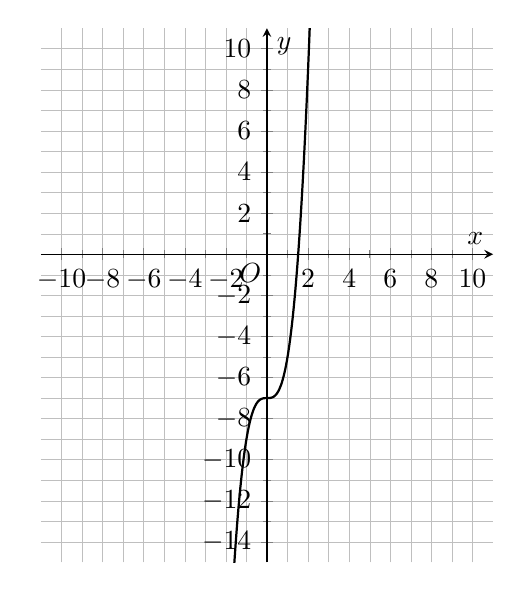
\begin{tikzpicture}
                            \begin{axis}[
                                    unit vector ratio*=1 1 1,
                                    axis lines = middle,
                                    xlabel = $x$,
                                    ylabel = $y$,
                                    ymin = -15,
                                    ymax = 11,
                                    xmin = -11,
                                    xmax = 11,
                                    xtick = {-10, -8,...,10},
                                    ytick = {-14,-12,...,10},
                                    minor tick num = 1,
                                    grid = both,
                                    grid style = {line width=.1pt, draw=gray!50},
                                    major grid style = {line width=.2pt,draw=gray!50},
                                    width = 0.8\textwidth,
                                ]
                                \node at (axis cs: 0,0) [anchor=north east, xshift=0.05cm] {$O$};
                                \addplot [
                                    thick,
                                    domain=-2:3,
                                    samples=100,
                                ]
                                {2*x^3 - 7};
                            \end{axis}
                        \end{tikzpicture}
                    \end{center}
                    \newpage

              \item $f(x) = \sqrt{3x - 9}$
                    \sol{}
                    \begin{center}
                        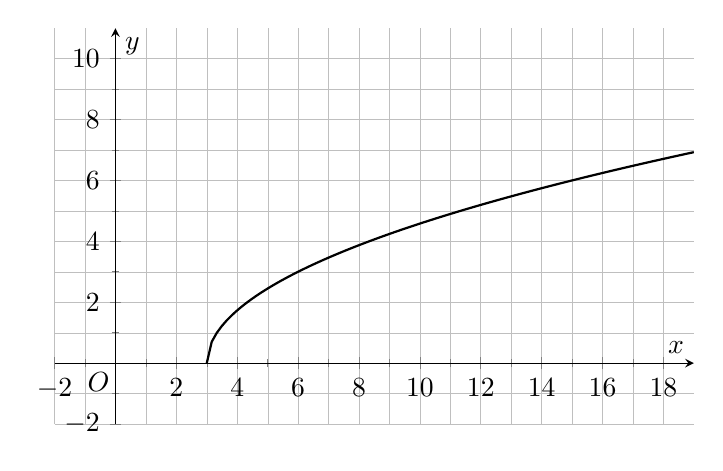
\begin{tikzpicture}
                            \begin{axis}[
                                    unit vector ratio*=1 1 1,
                                    axis lines = middle,
                                    xlabel = $x$,
                                    ylabel = $y$,
                                    ymin = -2,
                                    ymax = 11,
                                    xmin = -2,
                                    xmax = 19,
                                    xtick = {-2, 0,...,18},
                                    ytick = {-2,0,...,10},
                                    minor tick num = 1,
                                    grid = both,
                                    grid style = {line width=.1pt, draw=gray!50},
                                    major grid style = {line width=.2pt,draw=gray!50},
                                    width = 0.8\textwidth,
                                ]
                                \node at (axis cs: 0,0) [anchor=north east, xshift=0.05cm] {$O$};
                                \addplot [
                                    thick,
                                    domain=3:19,
                                    samples=100,
                                ]
                                {sqrt(3*x - 9)};
                            \end{axis}
                        \end{tikzpicture}
                    \end{center}

              \item $f(x) = \dfrac{4}{2x+11}$
                    \sol{}
                    \begin{center}
                        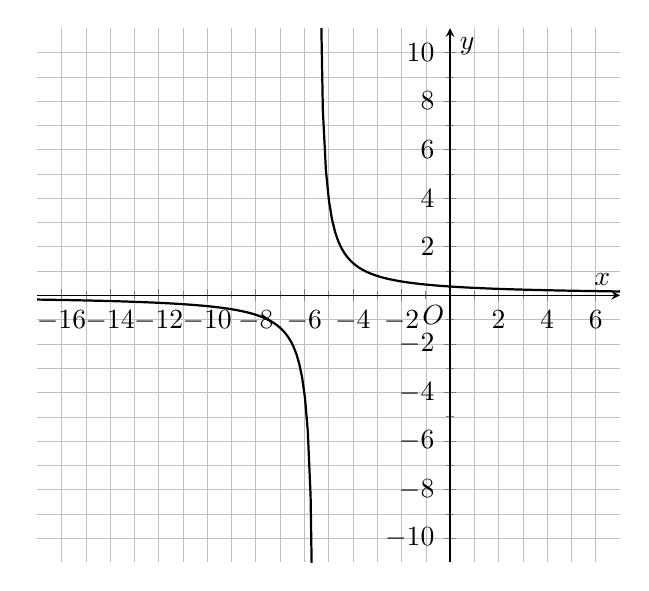
\begin{tikzpicture}
                            \begin{axis}[
                                    unit vector ratio*=1 1 1,
                                    axis lines = middle,
                                    xlabel = $x$,
                                    ylabel = $y$,
                                    ymin = -11,
                                    ymax = 11,
                                    xmin = -17,
                                    xmax = 7,
                                    xtick = {-16, -14,...,6},
                                    ytick = {-10,-8,...,10},
                                    minor tick num = 1,
                                    grid = both,
                                    grid style = {line width=.1pt, draw=gray!50},
                                    major grid style = {line width=.2pt,draw=gray!50},
                                    width = 0.8\textwidth,
                                ]
                                \node at (axis cs: 0,0) [anchor=north east, xshift=0.05cm] {$O$};
                                \addplot [
                                    thick,
                                    domain=-17:-5.51,
                                    samples=100,
                                ]
                                {4/(2*x+11)};
                                \addplot [
                                    thick,
                                    domain=-5.49:7,
                                    samples=100,
                                ]
                                {4/(2*x+11)};
                            \end{axis}
                        \end{tikzpicture}
                    \end{center}

                    \newpage
              \item $f(x) = \dfrac{2x + 7}{x-1}$
                    \sol{}
                    \begin{center}
                        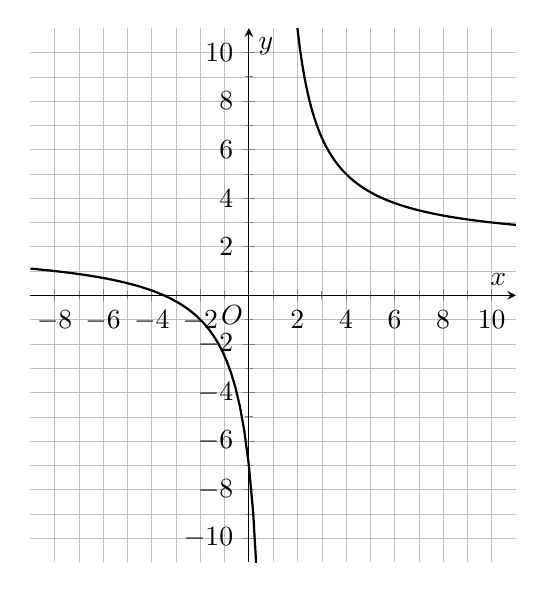
\begin{tikzpicture}
                            \begin{axis}[
                                    unit vector ratio*=1 1 1,
                                    axis lines = middle,
                                    xlabel = $x$,
                                    ylabel = $y$,
                                    ymin = -11,
                                    ymax = 11,
                                    xmin = -9,
                                    xmax = 11,
                                    xtick = {-8, -6,...,10},
                                    ytick = {-10,-8,...,10},
                                    minor tick num = 1,
                                    grid = both,
                                    grid style = {line width=.1pt, draw=gray!50},
                                    major grid style = {line width=.2pt,draw=gray!50},
                                    width = 0.8\textwidth,
                                ]
                                \node at (axis cs: 0,0) [anchor=north east, xshift=0.05cm] {$O$};
                                \addplot [
                                    thick,
                                    domain=-17:0.9,
                                    samples=100,
                                ]
                                {(2*x + 7)/(x-1)};
                                \addplot [
                                    thick,
                                    domain=1.1:11,
                                    samples=100,
                                ]
                                {(2*x + 7)/(x-1)};
                            \end{axis}
                        \end{tikzpicture}
                    \end{center}

              \item $f(x) = 2\sqrt{x+5} - 4$
                    \sol{}
                    \begin{center}
                        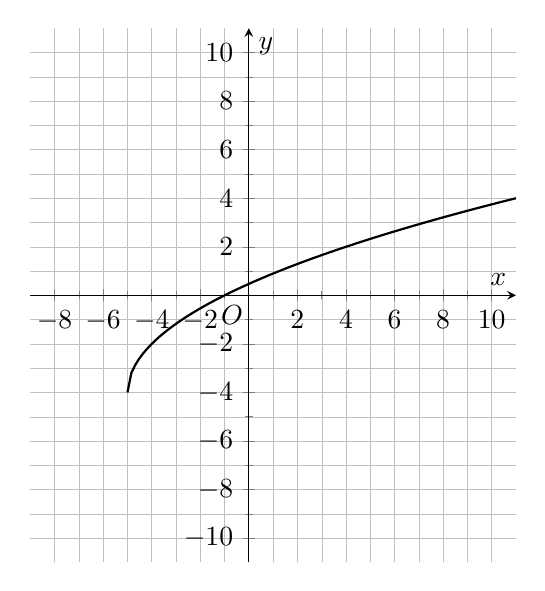
\begin{tikzpicture}
                            \begin{axis}[
                                    unit vector ratio*=1 1 1,
                                    axis lines = middle,
                                    xlabel = $x$,
                                    ylabel = $y$,
                                    ymin = -11,
                                    ymax = 11,
                                    xmin = -9,
                                    xmax = 11,
                                    xtick = {-8, -6,...,10},
                                    ytick = {-10,-8,...,10},
                                    minor tick num = 1,
                                    grid = both,
                                    grid style = {line width=.1pt, draw=gray!50},
                                    major grid style = {line width=.2pt,draw=gray!50},
                                    width = 0.8\textwidth,
                                ]
                                \node at (axis cs: 0,0) [anchor=north east, xshift=0.05cm] {$O$};
                                \addplot [
                                    thick,
                                    domain=-5:11,
                                    samples=100,
                                ]
                                {2*sqrt(x+5) - 4};
                            \end{axis}
                        \end{tikzpicture}
                    \end{center}
              \item $f(x) = \dfrac{1}{(2x - 3)^2}$
                    \sol{}
                    \begin{center}
                        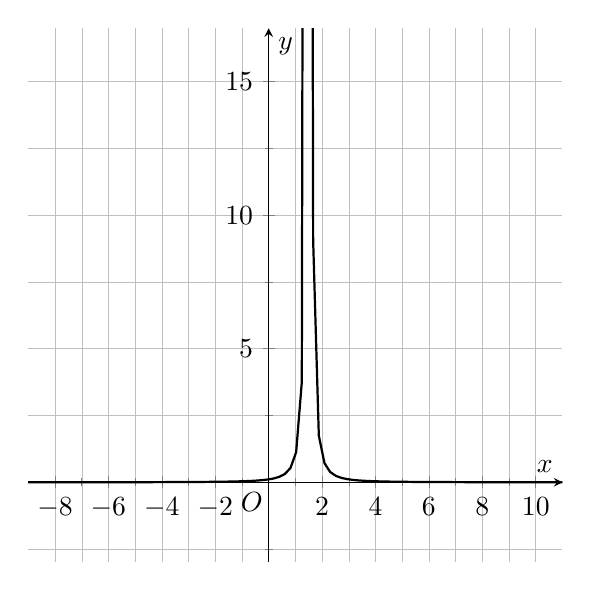
\begin{tikzpicture}
                            \begin{axis}[
                                    unit vector ratio*=1 1 1,
                                    axis lines = middle,
                                    xlabel = $x$,
                                    ylabel = $y$,
                                    ymin = -3,
                                    ymax = 17,
                                    xmin = -9,
                                    xmax = 11,
                                    xtick = {-8, -6,...,10},
                                    ytick = {-2,-8,...,16},
                                    minor tick num = 1,
                                    grid = both,
                                    grid style = {line width=.1pt, draw=gray!50},
                                    major grid style = {line width=.2pt,draw=gray!50},
                                    width = 0.8\textwidth,
                                ]
                                \node at (axis cs: 0,0) [anchor=north east, xshift=0.05cm] {$O$};
                                \addplot [
                                    thick,
                                    domain=-10:11,
                                    samples=100,
                                ]
                                {1/(2*x - 3)^2};
                            \end{axis}
                        \end{tikzpicture}
                    \end{center}

              \item $f(x) = \left\{\begin{array}{rl}
                            2x + 1, & x < 0    \\
                            x^2,    & x \geq 0
                        \end{array}\right.$
                    \sol{}
                    \begin{center}
                        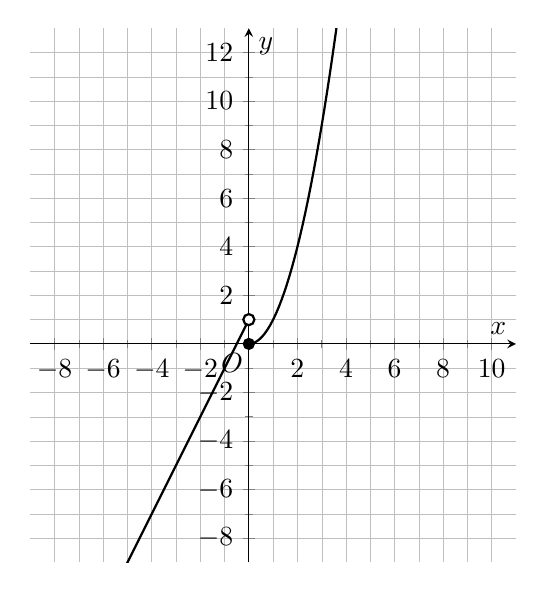
\begin{tikzpicture}
                            \begin{axis}[
                                    unit vector ratio*=1 1 1,
                                    axis lines = middle,
                                    xlabel = $x$,
                                    ylabel = $y$,
                                    ymin = -9,
                                    ymax = 13,
                                    xmin = -9,
                                    xmax = 11,
                                    xtick = {-8, -6,...,10},
                                    ytick = {-8,-6,...,12},
                                    minor tick num = 1,
                                    grid = both,
                                    grid style = {line width=.1pt, draw=gray!50},
                                    major grid style = {line width=.2pt,draw=gray!50},
                                    width = 0.8\textwidth,
                                ]
                                \node at (axis cs: 0,0) [anchor=north east, xshift=0.05cm] {$O$};
                                \addplot [
                                    thick,
                                    domain=-10:0,
                                    samples=100,
                                ]
                                {2*x + 1};
                                \addplot [
                                    thick,
                                    domain=0:11,
                                    samples=100,
                                ]
                                {x^2};

                                \filldraw[black] (axis cs:0,0) circle (2pt);
                                \filldraw[thick, fill=white] (axis cs:0,1) circle (2pt);
                            \end{axis}
                        \end{tikzpicture}
                    \end{center}
              \item $f(x) = \left\{\begin{array}{rl}
                            1 - x^2,      & x \leq 1 \\
                            x^2 + 2x - 3, & x > 1
                        \end{array}\right.$
                    \sol{}
                    \begin{center}
                        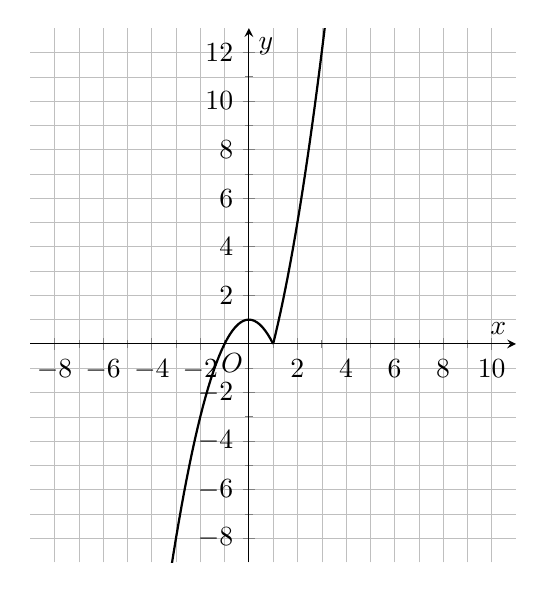
\begin{tikzpicture}
                            \begin{axis}[
                                    unit vector ratio*=1 1 1,
                                    axis lines = middle,
                                    xlabel = $x$,
                                    ylabel = $y$,
                                    ymin = -9,
                                    ymax = 13,
                                    xmin = -9,
                                    xmax = 11,
                                    xtick = {-8, -6,...,10},
                                    ytick = {-8,-6,...,12},
                                    minor tick num = 1,
                                    grid = both,
                                    grid style = {line width=.1pt, draw=gray!50},
                                    major grid style = {line width=.2pt,draw=gray!50},
                                    width = 0.8\textwidth,
                                ]
                                \node at (axis cs: 0,0) [anchor=north east, xshift=0.05cm] {$O$};
                                \addplot [
                                    thick,
                                    domain=-10:1,
                                    samples=100,
                                ]
                                {1 - x^2};
                                \addplot [
                                    thick,
                                    domain=1:11,
                                    samples=100,
                                ]
                                {x^2 + 2*x - 3};

                            \end{axis}
                        \end{tikzpicture}
                    \end{center}
          \end{enumerate}

    \item Given the function $f:x \to 2x^2$ and $g:x \to 3x - 4$. Find the value of $m$
          such that $(f \circ g)(m) = (g \circ f)(m)$. \sol{}
          \begin{align*}
              (f \circ g)(m)       & = (g \circ f)(m)  \\
              f(g(m))              & = g(f(m))         \\
              f(3m - 4)            & = g(2m^2)         \\
              2(3m - 4)^2          & = 3(2m^2) - 4     \\
              18m^2 - 48m + 32     & = 6m^2 - 4        \\
              12m^2 - 48m + 36     & = 0               \\
              3m^2 - 12m + 9       & = 0               \\
              (3m - 3)(m - 3)      & = 0               \\
              m                = 3 & \text{ or } m = 1
          \end{align*}

          \newpage

    \item Given the function $f:x \to x^2 + 2x - 3$ and $g:x \to 3x - 4$. If $(f \circ
              g)(k) = (g \circ f)(k)$, find the value of $k$. \sol{}
          \begin{flalign*}
              (f \circ g)(k)               & = (g \circ f)(k)      \\
              f(g(k))                      & = g(f(k))             \\
              f(3k - 4)                    & = g(k^2 + 2k - 3)     \\
              (3k - 4)^2 + 2(3k - 4) - 3   & = 3(k^2 + 2k - 3) - 4 \\
              9k^2 - 24k + 16 + 6k - 8 - 3 & = 3k^2 + 6k - 9 - 4   \\
              9k^2 - 18k + 5               & = 3k^2 + 6k - 13      \\
              6k^2 - 24k + 18              & = 0                   \\
              k^2 - 4k + 3                 & = 0                   \\
              (k - 3)(k - 1)               & = 0                   \\
              k = 3                        & \text{ or } k = 1
          \end{flalign*}

    \item Given that $f(x) = 3x + 1$, $x \neq 0$. If $(f \circ g)(x) = 6x^2 - 9x + 4$,
          find $g(x)$. \sol{}
          \begin{flalign*}
              (f \circ g)(x) & = 6x^2 - 9x + 4 \\
              f(g(x))        & = 6x^2 - 9x + 4 \\
              3g(x) + 1      & = 6x^2 - 9x + 4 \\
              3g(x)          & = 6x^2 - 9x + 3 \\
              g(x)           & = 2x^2 - 3x + 1
          \end{flalign*}

    \item Given that $f(x) = \dfrac{x+1}{x}$, $x \neq 0$. If $(f \circ g)(x) = x$, find
          $g(x)$. \sol{}
          \begin{flalign*}
              (f \circ g)(x)        & = x                                \\
              f(g(x))               & = x                                \\
              \frac{g(x) + 1}{g(x)} & = x                                \\
              g(x) + 1              & = xg(x)                            \\
              g(x) - xg(x)          & = -1                               \\
              g(x)(1 - x)           & = -1                               \\
              g(x)                  & = \frac{-1}{1 - x}                 \\
                                    & = \frac{1}{x - 1} \quad (x \neq 1)
          \end{flalign*}

    \item A function $f$ is defined by $f: x \to x - 3$. Find another function $g$ such
          that $g\circ f: x\to 4x^2 - 20x + 25$. \sol{}
          \begin{flalign*}
              (g \circ f)(x) & = 4x^2 - 20x + 25 \\
              g(f(x))        & = 4x^2 - 20x + 25 \\
              g(x - 3)       & = 4x^2 - 20x + 25
          \end{flalign*}
          \vspace{-1.2cm}
          \begin{flalign*}
              \text{Let } y & = x - 3 \\
              x             & = y + 3
          \end{flalign*}
          \vspace{-1.2cm}
          \begin{flalign*}
              g(y)             & = 4(y + 3)^2 - 20(y + 3) + 25     \\
                               & = 4(y^2 + 6y + 9) - 20y - 60 + 25 \\
                               & = 4y^2 + 24y + 36 - 20y - 35      \\
                               & = 4y^2 + 4y + 1                   \\
                               & = (2y + 1)^2                      \\
              \\
              \therefore\ g(x) & = (2x + 1)^2
          \end{flalign*}

    \item Let $f: \mathbb{R} \to \mathbb{R}$ be defined by $f(x) = \left\{\begin{array}{rl}
                  -2,       & x\leq -3   \\
                  |x| - 2x, & -3 < x < 3 \\
                  2x - 1,   & x \geq 3
              \end{array}\right.$. Find $(f \circ f \circ f)(-1000).$
          \sol{}
          \begin{flalign*}
              (f \circ f \circ f)(-1000) & = f(f(f(-1000)))  \\
                                         & = f(f(-2))        \\
                                         & = f(|-2| - 2(-2)) \\
                                         & = f(2 + 4)        \\
                                         & = f(6)            \\
                                         & = 2(6) - 1        \\
                                         & = 11
          \end{flalign*}

          \newpage
    \item Let function $f: A \to \mathbb{R}$ be defined by $f: x \to 2x^2$. Determine if
          $f$ is one to one function when $A$ is the following sets.
          \begin{enumerate}
              \item $A = \left\{x | 0 \leq x < 6\right\}$
              \item $A = \left\{x | x < 0\right\}$
              \item $A = \left\{x | -2 \leq x < 2\right\}$
              \item $A = \left\{x | x > 3\right\}$
          \end{enumerate}

    \item Determine whether the following functions are one to one functions or onto
          functions.
          \begin{enumerate}
              \item $f: \mathbb{R}^+ \to \mathbb{R}$, $f:x \to |x|-2$
              \item $f: \mathbb{R}\setminus\left\{2\right\} \to \mathbb{R}\setminus\left\{1\right\}$, $f:x \to \dfrac{x}{x-2}$
              \item $f: \mathbb{R} \to \mathbb{R}^+\cup\left\{0\right\}$, $f:x \to |x|$
          \end{enumerate}

    \item Let $A = \mathbb{R} \setminus \left\{-\dfrac{1}{2}\right\}$ and $A = \mathbb{R}
              \setminus \left\{\dfrac{1}{2}\right\}$, function $f: A \to B$ is defined by
          $f(x) = \dfrac{x-3}{2x + 1}$. Find
          \begin{enumerate}
              \item $f^{-1}(-2)$
              \item $f^{-1}(0)$
              \item $f^{-1}(3)$
          \end{enumerate}

    \item Let function $f: \mathbb{R}^+ \to \mathbb{R}^+$ be defined by $f(x) = x^2 + 2x
              + 1$. Find $f^{-1}(4)$ and $f^{-1}(9)$.

    \item A function $f$ is defined by $f:x \to \dfrac{x}{2} + 1$. If $g \circ f^{-1}: x
              \to 4x^2 - 8x + 7$, find the function $g$.

    \item Given the functioon $f:x \to 3x^2 + 5x + 9$, $x \leq a$. Find the maximum value
          of $a$ such that the inverse function of $f$ exists.

    \item Let the function $f$ and $g$ be defined as $f:x \to 5x + 3$ and $g:x \to 2x -
              7$ respectively. Find
          \begin{enumerate}
              \item $f \circ g$
              \item $f^{-1}$
              \item $g^{-1}$
          \end{enumerate}

    \item Given the function $f:x \to 2x + 3$ and $g:x \to {3-x}{2x + 5}$, $x \neq
              -\dfrac{5}{2}$. Find
          \begin{enumerate}
              \item $f \circ g$
              \item $f^{-1}$
              \item $g^{-1}$
          \end{enumerate}
          Show that $g^{-1} \circ f^{-1} = (f \circ g)^{-1}$.

    \item Given the function $f:x \to \sqrt{x}$, $x \neq 0$ and $g:x \to x^3$. Find
          \begin{enumerate}
              \item $g \circ f$
              \item $f^{-1}$
              \item $g^{-1}$
              \item $(g \circ f)^{-1}$
              \item $g^{-1} \circ f^{-1}$
          \end{enumerate}

    \item Given the function $f:x \to 2\sqrt{x-4} + 3$, $x \geq 4$.
          \begin{enumerate}
              \item Find the range of $f$.
              \item Find the inverse function $f^{-1}$ of $f$.
              \item On the same diagram, sketch the graphs of $f$ and $f^{-1}$.
          \end{enumerate}

\end{enumerate}
\end{document}